%
% teil1.tex -- Beispiel-File für das Paper
%
% (c) 2020 Prof Dr Andreas Müller, Hochschule Rapperswil
%
\section{Lösung
\label{parzyl:section:teil1}}
\rhead{Lösung}

\eqref{parzyl:sep_dgl_3} beschriebt einen ungedämpften harmonischen Oszillator.
Die Lösung ist somit
\begin{equation}
	i(z) 
	= 
	A\cos{ 
		\left ( 
		\sqrt{\lambda + \mu}z
		\right )}
	+
	B\sin{ 
		\left ( 
		\sqrt{\lambda + \mu}z
		\right )}.
\end{equation}
Die Differentialgleichungen \eqref{parzyl:sep_dgl_1} und \eqref{parzyl:sep_dgl_2} werden in \cite{parzyl:whittaker}
mit Hilfe der Whittaker Gleichung gelöst.
\begin{definition}
    Die Funktion 
    \begin{equation*}
        W_{k,m}(z) = 
    e^{-z/2} z^{m+1/2} \,
    {}_{1} F_{1}
    (
        {\textstyle \frac{1}{2}} 
        + m - k, 1 + 2m; z)
    \end{equation*}
    heisst Whittaker Funktion und ist eine Lösung
    von der Whittaker Differentialgleichung
    \begin{equation}
        \frac{d^2W}{d z^2} +
        \left(-\frac{1}{4}  + \frac{k}{z} + \frac{\frac{1}{4} - m^2}{z^2} \right) W = 0.
        \label{parzyl:eq:whitDiffEq}
    \end{equation}
\end{definition}
Es wird nun die Differentialgleichung bestimmt, welche
\begin{equation}
    w = z^{-1/2} W_{k,-1/4} \left({\textstyle \frac{1}{2}} z^2\right)
\end{equation}
als Lösung hat.
Dafür wird $w$ in \eqref{parzyl:eq:whitDiffEq} eingesetzt woraus
\begin{equation}
    \frac{d^2 w}{dz^2} - \left(\frac{1}{4} z^2 - 2k\right) w = 0
\label{parzyl:eq:weberDiffEq}
\end{equation}
resultiert. DIese Differentialgleichung ist dieselbe wie 
\eqref{parzyl:sep_dgl_2} und \eqref{parzyl:sep_dgl_2}, welche somit
$w$ als Lösung haben.
Da es sich um eine Differentialgleichung zweiter Ordnung handelt, hat sie nicht nur
eine sondern zwei Lösungen.
Die zweite Lösung der Whittaker-Gleichung ist $W_{k,-m} (z)$.
Somit hat \eqref{parzyl:eq:weberDiffEq}
\begin{align}
    w_1(k, z) & = z^{-1/2} W_{k,-1/4} \left({\textstyle \frac{1}{2}} z^2\right)\\
    w_2(k, z) & = z^{-1/2} W_{k,1/4} \left({\textstyle \frac{1}{2}} z^2\right)
\end{align}
als Lösungen.
Mit der Hypergeometrischen Funktion ausgeschrieben ergeben sich die Lösungen
\begin{align}
	\label{parzyl:eq:solution_dgl}
    w_1(k,z) &= e^{-z^2/4} \,
    {}_{1} F_{1}
    (
        {\textstyle \frac{1}{4}} 
         - k, {\textstyle \frac{1}{2}} ; {\textstyle \frac{1}{2}}z^2) \\
    w_2(k,z) & = z e^{-z^2/4} \,
         {}_{1} F_{1}
         ({\textstyle \frac{3}{4}} 
              - k, {\textstyle \frac{3}{2}} ; {\textstyle \frac{1}{2}}z^2).
\end{align}
In der Literatur gibt es verschiedene Standartlösungen für $w(k,z)$ präsentiert.
Whittaker und Watson zeigen in \cite{parzyl:whittaker} eine Lösung
\begin{equation}
    D_n(z) = \frac{
            \Gamma \left( {\textstyle \frac{1}{2}}\right) 2^{\frac{1}{2}n + \frac{1}{2}} z^{-\frac{1}{2}}
        }{
            \Gamma \left( {\textstyle \frac{1}{2}} \right) - {\textstyle \frac{1}{2}} n)
        }
        M_{\frac{1}{2} n + \frac{1}{4}, - \frac{1}{4}} \left(\frac{1}{2}z^2\right)
        +
        \frac{
            \Gamma\left(-{\textstyle \frac{1}{2}}\right) 2^{\frac{1}{2}n + \frac{1}{4}} z^{-\frac{1}{2}}
        }{
            \Gamma\left(- {\textstyle \frac{1}{2}} n\right)
        }
        M_{\frac{1}{2} n + \frac{1}{4}, \frac{1}{4}} \left(\frac{1}{2}z^2\right)
\end{equation}
welche die Differentialgleichung
\begin{equation}
    \frac{d^2D_n(z)}{dz^2} + \left(n + \frac{1}{2} - \frac{1}{4} z^2\right)D_n(z) = 0
\end{equation}
löst.

In \cite{parzyl:abramowitz-stegun} sind zwei Lösungen $U(a, z)$ und $V(a,z)$ 
\begin{align}
    U(a,z) &= 
    \cos\left[\pi \left({\textstyle \frac{1}{4}} + {\textstyle \frac{1}{2}} a\right)\right] Y_1
    - \sin\left[\pi \left({\textstyle \frac{1}{4}} + {\textstyle \frac{1}{2}} a\right)\right] Y_2 \\
    V(a,z) &= \frac{1}{\Gamma \left({\textstyle \frac{1}{2} - a}\right)} \left\{
    \sin\left[\pi \left({\textstyle \frac{1}{4}} + {\textstyle \frac{1}{2}} a\right)\right] Y_1
    + \cos\left[\pi \left({\textstyle \frac{1}{4}} + {\textstyle \frac{1}{2}} a\right)\right] Y_2
    \right\}
\end{align}
mit
\begin{align}
    Y_1 &= \frac{1}{\sqrt{\pi}} 
            \frac{\Gamma\left({\textstyle \frac{1}{4} - 
            {\textstyle \frac{1}{2}}a}\right)}
            {2^{\frac{1}{2} a + \frac{1}{4}}} w_1\\
    Y_2 &= \frac{1}{\sqrt{\pi}} 
            \frac{\Gamma\left({\textstyle \frac{3}{4} - 
            {\textstyle \frac{1}{2}}a}\right)}
            {2^{\frac{1}{2} a - \frac{1}{4}}} w_2
\end{align}
der Differentialgleichung
\begin{equation}
    \frac{d^2 y}{d z^2} - \left(\frac{1}{4} z^2 + a\right) y = 0
\end{equation}
beschrieben. Die Lösungen $U(a,z)$ und $V(a, z)$ können auch mit $D_n(z)$
ausgedrückt werden
\begin{align}
    U(a,z) &= D_{-a-1/2}(z) \\
    V(a,z) &= \frac{\Gamma \left({\textstyle \frac{1}{2}} + a\right)}{\pi}
    \left[\sin\left(\pi a\right) D_{-a-1/2}(z) + D_{-a-1/2}(-x)\right].
\end{align}
TODO Plot
\begin{figure}
    \centering
    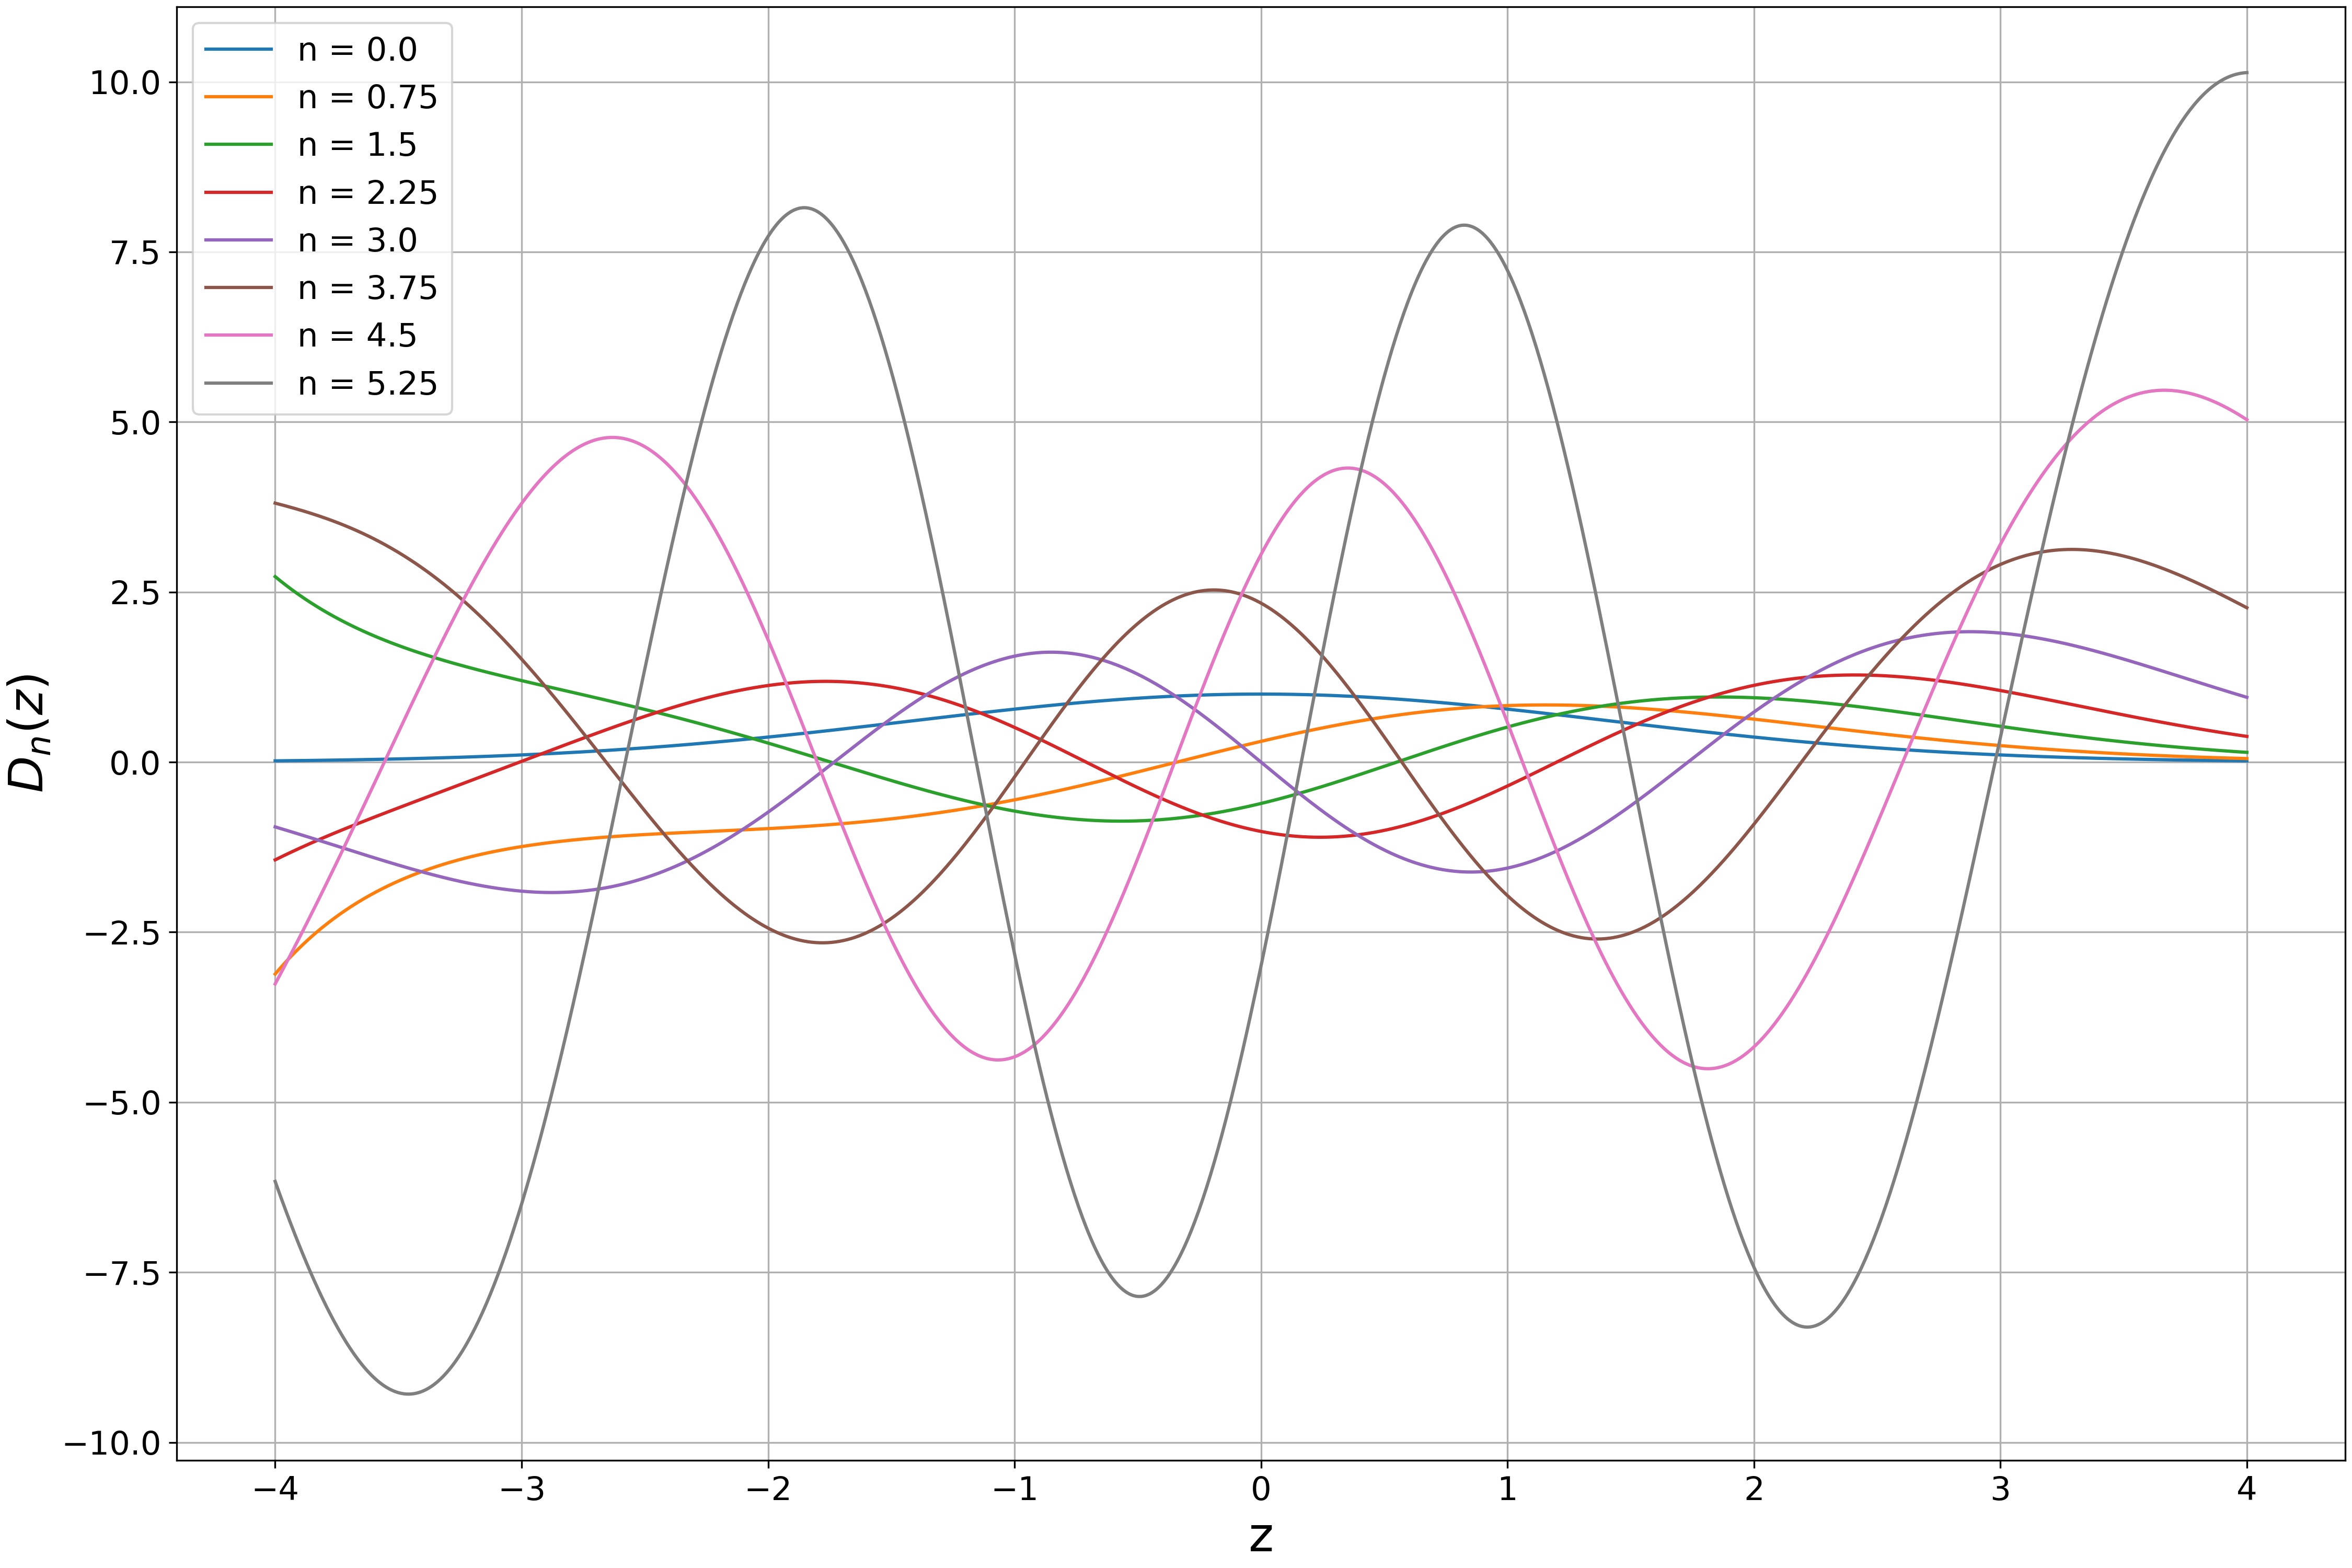
\includegraphics[scale=0.3]{papers/parzyl/img/D_plot.png}
    \caption{$D_a(z)$ mit unterschiedlichen Werten für $a$.}
    \label{parzyl:fig:dnz}
\end{figure}
\begin{figure}
    \centering
    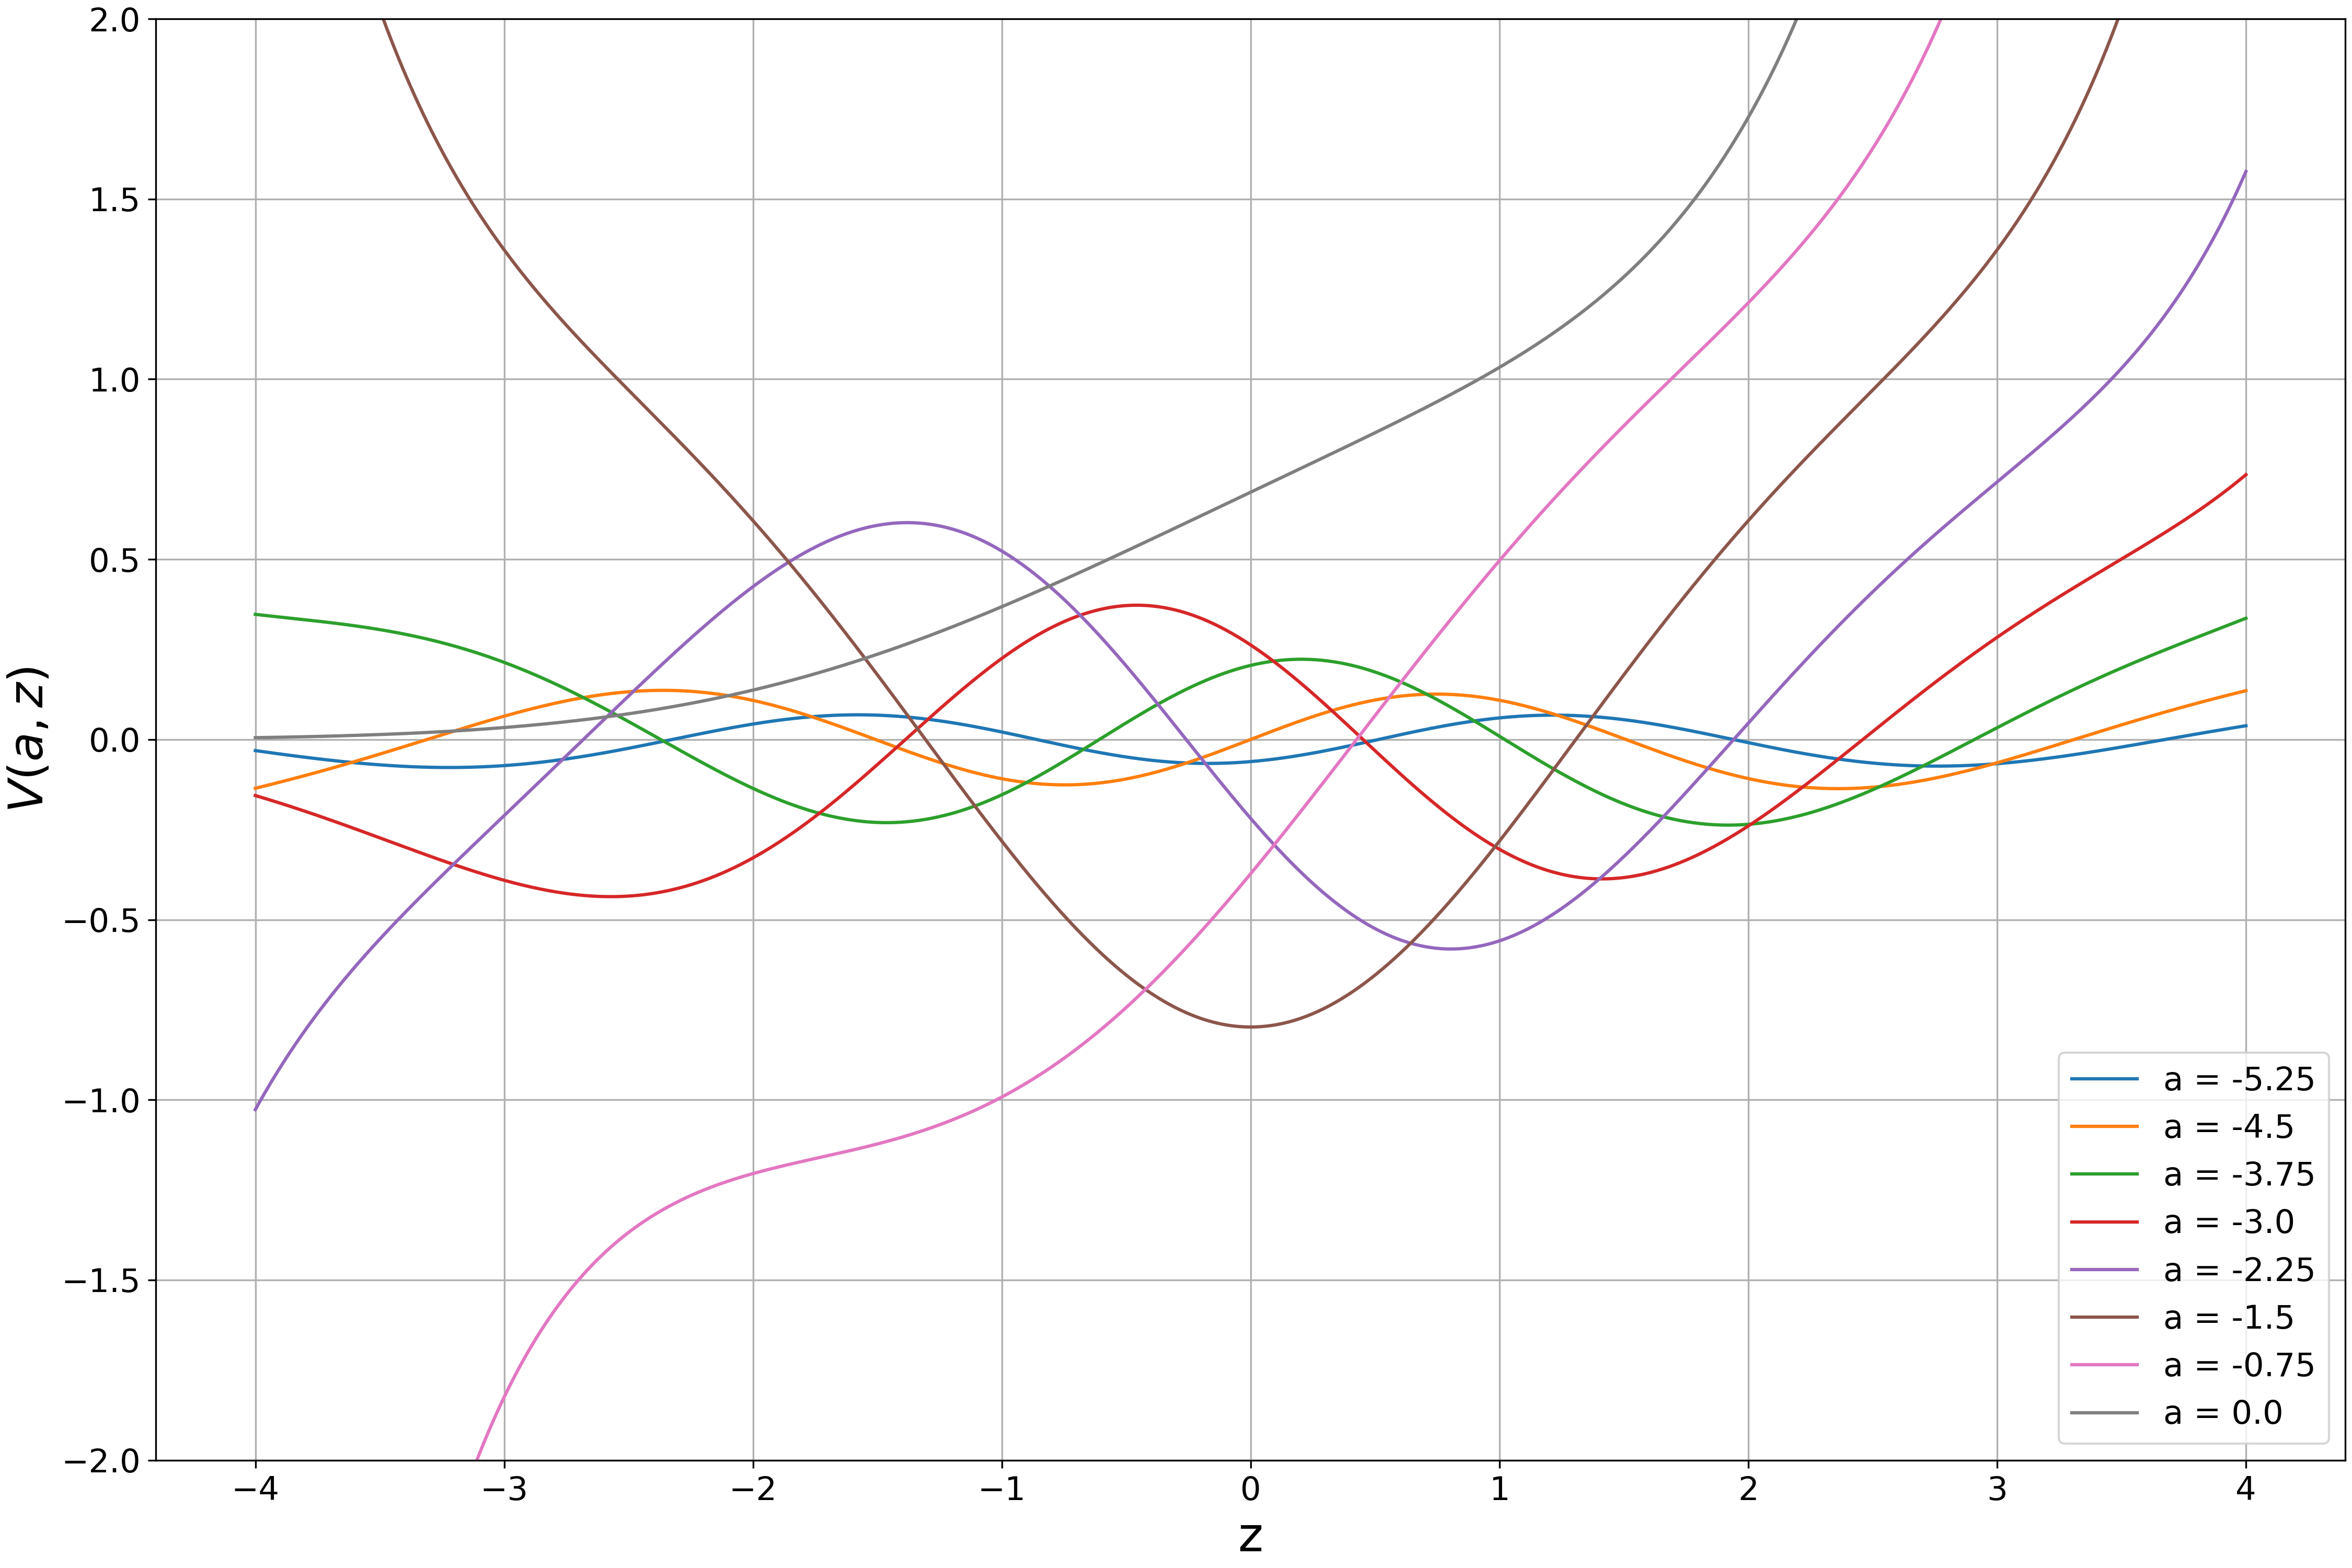
\includegraphics[scale=0.3]{papers/parzyl/img/v_plot.png}
    \caption{$V(a,z)$ mit unterschiedlichen Werten für $a$.}
    \label{parzyl:fig:Vnz}
\end{figure}